
	\subsection{Herramientas de simulaci\'on}		
	El prop\'osito central de este proyecto es encontrar un modelo con estrutuctura de \'arbol que sea capaz de invertir en bolsa de forma beneficiosa. Puesto que la ejecuci\'on del modelo es necesaria para medir su bondad, hay que trabajar en un entorno de pruebas en el que poder hacer ensayos. Este entorno no debe ser la bolsa real, porque simular grandes periodos costar\'ia el mismo tiempo que la longitud del periodo y, adem\'as, se estar\'ia haciendo con dinero real, con todas las dificultades que esto puede tener.\\
	
	En su lugar, las plataformas de \textit{backtesting} ofrecen las simulaciones que se necesitan. El \textit{backtesting} es el proceso que permite simular un periodo de bolsa e invertir con una estrategia particular de forma sistem\'atica. A continuaci\'on, se mencionan algunas plataformas y un peque\~no an\'alisis de cada una para discernir cu\'al es mejor para esta tarea. 
	
	
		\subsubsection{MetaTrader5}
		
    	\textit{MetaTrader5} es una software, disponible en versi\'on escritorio y en versi\'on web, con el que se pueden comprar y vender acciones en tiempo real pero de forma simulada, es decir, sin participar con dinero real. Es una plataforma ampliamente usada y, por tanto, es f\'acil encontrar ejemplos iniciales o ayuda t\'ecnica. Por comentar una de las facilidades, en la p\'agina web de la plataforma\footnote{\url{https://www.metatrader5.com} [\'Ultima consulta 10 de Julio de 2019]} se nos ofrece una demo gratuita con acceso a la mayor\'ia de los recursos, aunque hay algunas herramientas de pago.
		
		La programaci\'on de las estrategias se organiza en varios archivos con unas especificaciones concretas. Adem\'as, existe una tienda empotrada en la plataforma para comprar y vender estrategias, \'indices o bibliotecas con otros usuarios. Cada producto est\'a puntuado por los usuarios que lo han usado. A priori, esto puede ser bastante \'util para comparar la estrategia propuesta en el proyecto con otras estrategias cl\'asicas o con las estrategias mejor puntuadas en la plataforma.\\
		
		A pesar de todas estas ventajas, no usaramos \textit{MetaTrader5} por ser de car\'acter privativo. Asimismo, el lenguaje de programaci\'on de las estrategias es \textit{MQL5}, un lenguaje propio de la plataforma, que nos impide usar con facilidad bibliotecas externas.
	
		\subsubsection{Backtrader}\label{sec:backtrader}
		
		\textit{Backtrader} es un \textit{framework} de libre licencia desarrollado en el lenguaje \textit{Python}. La p\'agina web de la plataforma\footnote{\url{https://www.backtrader.com} [\'Ultima consulta 10 de Julio de 2019]} contiene una amplia documentaci\'on en la que se explican todos los componentes de este \textit{framework}. Tambi\'en se encuentran, en el mismo lugar, el m\'etodo de instalaci\'on y un tutorial de iniciaci\'on para simulaci\'on de bolsa.
		
		La herramienta contiene indicadores ya programados, aunque se permite hacer m\'as de forma manual.  Instalando una librer\'ia adicional se pueden generar gr\'aficas de ganancias en un periodo de simulaci\'on. Este desacoplamiento de la parte gr\'afica no supone un gran problema porque en la instalaci\'on viene integrada la opci\'on para instalar todo, tal y como se ver\'a en el siguiente apartado.\\
		
		
		\paragraph{Instalaci\'on}\label{sec:install}
		
		Pasamos pues, a ilustrar la instalaci\'on de \textit{backtrader}. La instalaci\'on puede hacerse en cualquier sistema operativo que soporte \textit{Python} pero, en lo que sigue, se supondr\'a que el sistema es \textit{Ubuntu}. 
		
		En primer lugar, es preciso tener la versi\'on 2.7 de \textit{Python}, como se indica en la documentaci\'on de \textit{backtrader}\footnote{\url{https://www.backtrader.com/docu/index.html} [\'Ultima consulta 10 de Julio de 2019]} que se ubica en su p\'agina web. Para comprobar la versi\'on, se puede usar el comando \textit{python -Version}. En caso de no tener instalado \textit{Python} o no tener la versi\'on indicada, se puede instalar usando \textit{sudo apt-get install python2.7}.\\
		
		El \textit{framework backtrader} est\'a disponible desde el c\'odigo fuente en \textit{Github}. No obstante, es m\'as c\'omodo usar la versi\'on para el instalador de paquetes de \textit{Python, pip}. Si no se tiene instalado \textit{pip}, la instalaci\'on se realiza con el comando \textit{sudo apt-get install python-pip}.\\
		
		Una vez llegados a este punto, se puede optar por una versi\'on con posibilidad de generar gr\'aficas o una versi\'on m\'as ligera sin esta posibilidad. Para facilitar el an\'alisis de resultados, se recomienda instalar la versi\'on con gr\'aficas. Su instalaci\'on se ejecuta con el comando \textit{pip install backtrader[plotting]}, como podemos ver en la figura \ref{fig:pip_backtrader}. Para instalar una versi\'on m\'as ligera, se usa el mismo comando quitando la directiva \textit{[plotting]}. En este caso se instala una versi\'on similar pero sin la posibilidad de hacer gr\'aficas.\\
		
		\begin{figure}[H]
			\centering
			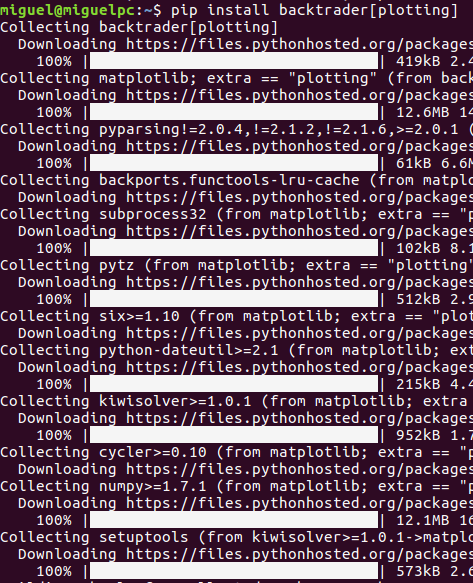
\includegraphics[scale=0.4]{imagenes/pip_backtrader.png}
			\caption[Resultado de instalar backtrader con plotting]{Resultado de instalar backtrader con plotting.\\ Fuente: elaboraci\'on propia.}
			\label{fig:pip_backtrader}
		\end{figure}
		
		La instalaci\'on de backtrader conlleva la instalaci\'on de otros paquetes adicionales con los que tiene dependencias. Entre ellos hay que destacar el paquete \textit{numpy}, que m\'as tarde nos ser\'a \'util como herramienta matem\'atica para generar distribuciones estad\'isticas.
		
		
		\paragraph{Preparaci\'on del entorno}
		
		Una de las estructuras de datos m\'as comunes en \textit{backtrader} son las l\'ineas. Una l\'inea no es m\'as que un conjunto de datos ordenados por orden cronol\'ogico, del m\'as antiguo al m\'as moderno. Por ejemplo, al hablar de un valor de mercado tenemos 5 l\'ineas b\'asicas: valor de apertura, valor de salida, valor m\'aximo, valor m\'inimo y volumen de compra/venta. 
		
		En t\'erminos de inform\'atica, para acceder a los elementos de cada l\'inea, hay que tener en cuenta que no se puede usar la indexaci\'on de un vector como en un lenguaje de programaci\'on com\'un. En su lugar, el \'indice 0 representa el instante actual y, a partir de este, se cuentan con los n\'umeros enteros las posiciones de los dem\'as. Hay que aclarar que para acceder a instantes anteriores usaremos \'indices negativos, como por ejemplo:
		
		\begin{lstlisting}[basicstyle=\tiny]
	self.sma = SimpleMovingAverage(...)
	valor_actual            = self.sma[0]
	valor_instante_anterior = self.sma[-1]
		\end{lstlisting}
		
		\vspace{0.8cm}
		
		Por tanto, seg\'un el d\'ia que se est\'e simulando, los datos de otro d\'ia concreto se acceden con un \'indice o con otro. De esta forma, suponiendo que se est\'a simulando el lunes y queremos acceder al dato del mi\'ercoles el \'indice es el 2. Si por el contrario se simula el jueves, para acceder al mi\'ercoles se usa el \'indice -1. N\'otese que, por motivos acad\'emicos, no se deben usar los \'indices mayores que 0, ya que esto supondr\'ia tener informaci\'on sobre el futuro y la predicci\'on de la bolsa ser\'ia un fraude.\\
		
		Antes de ver c\'omo crear una estrategia, es preciso ver como se puede simular una prueba introduciendo unos datos y un presupuesto inicial. Para ello, en un archivo con terminaci\'on \textit{.py}, para poder ejecutar con \textit{Python}, se insertar\'a el siguiente c\'odigo:
		
		\begin{lstlisting}[basicstyle=\tiny]
from __future__ import (absolute_import, division, print_function, unicode_literals)
		
import datetime
import os.path
import sys
import backtrader as bt # Importar todas las herramientas de backtrader
		
if __name__ == '__main__':
	cerebro = bt.Cerebro()
		
# Crear un paquete de datos
	data = bt.feeds.YahooFinanceCSVData(
	dataname='YAHOO',  # Ruta absoluta donde se encuentran los datos descargados de YAHOO! Finance
# Fecha inicial de los datos
	fromdate=datetime.datetime(2000, 1, 1),
# Fecha final de los datos
	todate=datetime.datetime(2000, 12, 31),
	reverse=False)
		
# Activar los datos en el cerebro
	cerebro.adddata(data)
# Establecer dinero inicial    
	cerebro.broker.setcash(100000.0)
		
	print('Starting Portfolio Value: %.2f' % cerebro.broker.getvalue())
	cerebro.run()   # EJECUTAR BACKTESTING (AHORA MISMO, SIN NINGUNA ESTRATEGIA)
	print('Final Portfolio Value: %.2f' % cerebro.broker.getvalue())
		\end{lstlisting}
		
		\vspace{0.5cm}
		
		N\'otese que se trata de una archivo \textit{Python} en el que solo hemos tenido que importar el paquete \textit{backtrader}. Por tanto, en el caso de necesitar otros paquetes para realizar nuestra estrategia, solo ser\'a necesario incorporarlos de la forma habitual en este lenguaje de programaci\'on.\\
		
		El c\'odigo es ejecutable y funcional, pero hay un problema, no se le ha especificado a la clase \textit{cerebro} cu\'al va a ser la estrategia a seguir. Por este motivo, si se haciera la simulaci\'on, el presupuesto inicial y final no variar\'ian. 
		
		Para ejecutar el \textit{backtesting} simplemente se ejecuta el \textit{script} de \textit{Python} con el comando \textit{python rutadelscript.py} en la terminal. Seguramente dar\'a un fallo porque la ruta donde deber\'ia estar el fichero con los datos a simular est\'a vac\'ia. Esto era de esperar pues no hemos descargado ning\'un archivo de datos. El desarrollo de este tema se abordar\'a en la secci\'on \ref{sec:get_data}.
		
		
		\paragraph{La primera estrategia}
		
		Antes de programar la primera estrategia de \textit{trading}, vamos a ilustrar con una f\'util c\'omo estructurar una clase para que \textit{backtrader} pueda trabajar con ella como estrategia. La estructura b\'asica es una clase con un m\'etodo \textit{\_\_init\_\_} y otro m\'etodo llamado \textit{next}. 
		
		El primero puede usarse para instanciar y agrupar los datos que requiera nuestra estrategia. El segundo m\'etodo, por su parte, es llamado en cada instante simulado por \textit{backtrader}, considerando que un instante es cada una de las marcas temporales que hay registradas en nuestros datos. Por aclarar esto un poco, si aportamos al \textit{cerebro} unos datos tomados de forma diaria, los instantes son cada uno de los d\'ias. \\
		
		Cabe destacar que, en cada llamada al segundo m\'etodo, solo son accesibles los datos con marcas temporales menores o iguales al instante correspondiente a la llamada. Existe, no obstante, una forma de saltarse esta regla y conseguir informaci\'on de instantes posteriores. Pero como se especific\'o en el apartado anterior, no es de inter\'es acad\'emico.\\
		
		Veamos un ejemplo b\'asico en el que, en cada instante, se imprime en pantalla el precio actual del valor:
		
		\begin{lstlisting}[basicstyle=\tiny]
# Crear una estrategia
class TestStrategy(bt.Strategy):

	def log(self, txt, dt=None):
		dt = dt or self.datas[0].datetime.date(0)
		print('%s, %s' % (dt.isoformat(), txt))
	
	def __init__(self):
	# Guarda una referencia de la linea de valores de cierre
		self.dataclose = self.datas[0].close
	
	def next(self):
	# Muestra por pantalla el valor de cierre
		self.log('Close, %.2f' % self.dataclose[0])
		\end{lstlisting}
		
		Al ejecutar el \textit{cerebro} con esta estrategia, veremos el valor de cierre de cada instante y, si los datos lo facilitan, la marca temporal asociada a cada instante.
		
		Para activar la estrategia es necesario indicar al \textit{cerebro} la clase creada con la siguiente l\'inea, que puede ser situada justo despu\'es de indicar el presupuesto inicial:

		\begin{lstlisting}[basicstyle=\tiny]
    # Registrar estrategia
    cerebro.addstrategy(TestStrategy)
		\end{lstlisting}	
		
		\vspace{0.4cm}
		
		De este modo, la estrategia est\'a completa, pero en ning\'un instante se realizan compras o ventas. Para nuestro posterior estudio es imprescindible introducir estas acciones. Sin embargo, por motivos de espacio y tiempo, no entraremos en profundidad en todos los aspectos de la compraventa.\\
		
		Veamos el c\'odigo de la primera t\'actica de inversi\'on que nos muestra el funcionamiento de las \'ordenes burs\'atiles:
		
		
		\begin{lstlisting}[basicstyle=\tiny]
class DoubleDownStrategy(bt.Strategy):

	def log(self, txt, dt=None):
		dt = dt or self.datas[0].datetime.date(0)
		print('%s, %s' % (dt.isoformat(), txt))

	def __init__(self):
		self.dataclose = self.datas[0].close

		# Para mantener las ordenes no ejecutadas
		self.order = None

	def notify_order(self, order):
		if order.status in [order.Submitted, order.Accepted]:
			return

		if order.status in [order.Completed]:
			if order.isbuy():
				self.log('BUY EXECUTED, %.2f' % order.executed.price)
			elif order.issell():
				self.log('SELL EXECUTED, %.2f' % order.executed.price)

			self.bar_executed = len(self)

		elif order.status in [order.Canceled, order.Margin, order.Rejected]:
			self.log('Order Canceled/Margin/Rejected')

		self.order = None

	def next(self):
		self.log('Close, %.2f' % self.dataclose[0])
		# Si hay una compraventa pendiente no puedo hacer otra
		if self.order:
			return

		# Si no tengo nada adquirido
		if not self.position:
			if self.dataclose[0] < self.dataclose[-1]:
				if self.dataclose[-1] < self.dataclose[-2]:
					self.log('BUY CREATE, %.2f' % self.dataclose[0])
					self.order = self.buy()

		else:
			# Ya hemos adquirido algo
			if len(self) >= (self.bar_executed + 5):
				self.log('SELL CREATE, %.2f' % self.dataclose[0])
				self.order = self.sell()
		\end{lstlisting}
		
		Aqu\'i se introducen varios conceptos nuevos del \textit{framework}. En primer lugar, las acciones \textit{self.buy()} y \textit{self.sell()}, ejecutadas dentro del m\'etodo \textit{next}, indican que queremos lanzar una orden de compra o de venta, respectivamente. Cuando no se especifica ning\'un par\'ametro, \textit{backtrader} compra o vende al precio de cierre del instante actual una sola acci\'on. Esto no quiere decir que la orden se ejecute en ese instante, sino que, a partir de ese momento y si el precio del producto lo permite, se realizar\'a lo antes posible. N\'otese que una vez lanzada una orden hay que esperar a que se complete o se cancele antes de lanzar otra.\\
		
		Seg\'un lo anterior, esta situaci\'on hace necesario incluir el m\'etodo \textit{notify\_order}. Como su propio nombre sugiere, es llamado cuando una orden cambia de estado o, en otras palabras, es el momento a partir del cual se puede lanzar una nueva orden. En este ejemplo, cuando una orden es completada, mostramos por pantalla si es de compra o venta y el precio de la misma. En ciertas ocasiones, las \'ordenes pueden terminar sin compra o venta. En ese caso, puede haber ocurrido una de dos: ser canceladas, si la estrategia cancel\'o la orden con el comando \textit{self.cancel()}, o rechazas, si bien el dinero disponible era insuficiente para ejecutar la orden.\\
		
		Por \'ultimo, comentaremos la parte l\'ogica de la estrategia presentada en el c\'odigo anterior. En cada instante, el m\'etodo \textit{next} eval\'ua alguno de los siguientes casos:
		
		\begin{itemize}
			\item \textbf{Existe una orden lanzada y no terminada.} En este caso debemos esperar. T\'engase en cuenta que \textit{backtrader} permite cancelar una orden, aunque no entraremos en este punto con profundidad.
			\item \textbf{No hay una orden lanzada y tampoco tengo nada comprado.} La cantidad de acciones que se poseen puede comprobarse con \textit{self.position}, que se interpreta como un booleano negativo si no se tiene nada en posesi\'on. En esta situaci\'on solo cabe esperar una orden de compra y, para nuestro ejemplo, la lanzaremos si los \'ultimos dos instantes han bajado su precio de cierre de forma consecutiva.
			\item \textbf{No hay una orden lanzada pero tengo algo comprado.} En este caso, se supone que solo se puede vender, aunque si se tuviese dinero no hay ning\'un problema en comprar m\'as acciones.
			
			 Para ilustrar una nueva herramienta, se propone lanzar una orden de venta cinco instantes despu\'es de haber comprado. Para ello podemos comprobar la longitud de \textit{self} con la funci\'on \textit{len} de \textit{Python}. Esta acci\'on, que puede resultar un tanto extra\~na, es una forma propia del lenguaje \textit{Python} de comprobar las dimensiones de un objeto, en este caso de la compra.
		\end{itemize}
		
		
		\subsubsection{Otras plataformas}

		\begin{itemize}
			\item \textbf{Tradestation.} Permite programar estrategias, pero no hacer \textit{backtesting}. Adem\'as no es de acceso gratuito y obliga a invertir con dinero real.
			
			\item \textbf{Cloud9trader.} Tiene una demo que permite programar estrategias y hacer \textit{backtesting}. Est\'a bien para probar estrategias sencillas basadas en indicadores ampliamente conocidos. No obstante, la programaci\'on hay que hacerla en la ventana del navegador, con un lenguaje propio y sin posibilidad de usar paquetes externos.
			
			\item \textbf{Plus500.} Es una plataforma de \textit{trading} con escasas posibilidades de automatizaci\'on. Tan solo permite algunas  sencillas \'ordenes condicionales preprogramadas.
			
			\item \textbf{PyAlgoTrade.} Es un proyecto desarrollado en \textit{Python} disponible en \textit{Github}. Tiene posibilidad de \textit{backtesting}, de utilizar paquetes externos y, en el caso de estar haciendo \textit{trading} con Bitcoins, de comprar y vender estos de forma real. Los datos del mercado hay que conseguirlos de forma externa en formato CSV.
		\end{itemize}
		
	
	\subsection{Conseguir datos hist\'oricos para realizar \textit{backtesting}}\label{sec:get_data}
		
		Como vamos a usar \textit{backtrader}, una herramienta de simulaci\'on de bolsa en local, vamos a necesitar extraer el hist\'orico de la bolsa. En esta secci\'on veremos c\'omo conseguir los valores hist\'oricos en bolsa de diferentes empresas de forma autom\'atica. A parte de conseguir los datos, veremos la forma de incorporarlos a backtrader para su posterior uso.
		
		\subsubsection{Quandl}
		
		\textit{Quandl} es una empresa que re\'une miles de paquetes de datos financieros de todo el mundo. Para acceder a esta informaci\'on es necesario registrarse en su p\'agina web. Una vez tengamos acceso, es posible descargar muchos de los archivos en formato CSV. Aunque quiz\'as la opci\'on m\'as c\'omoda para este proyecto sea utilizar la \textit{API} que ofrece. De esta forma se realiza el acceso a los datos desde \textit{Python}, sin necesidad de hacer una descarga previa a la ejecuci\'on del \textit{script}.\\
		
		Para usar la \textit{API} seguiremos los pasos de instalaci\'on que se pueden encontrar en la documentaci\'on\footnote{\url{https://docs.quandl.com/docs/python-installation} [\'Ultima consulta 10 de Julio de 2019]} de \textit{Quandl}. As\'i, instalamos el paquete \textit{quandl} con el gestor de paquetes \textit{pip}. No obstante, para usar el paquete, debemos indicar la \textit{api\_key} que nos dan al inscribirnos en su p\'agina, \'unica para cada usuario.\\
		
		\begin{lstlisting}[basicstyle=\tiny]
# Crear un paquete de datos con QUANDL
	data = bt.feeds.Quandl(
		dataset='WFE',
		fromdate = datetime.datetime(2016,1,1),
		todate = datetime.datetime(2017,1,1),
		dataname='INDEXES_BMESPANISHEXCHANGESMADRID',
		buffered=True,
		apikey='')
		\end{lstlisting}

			
			

		No obstante, como puede verse en la figura \ref{fig:quandl_install}, \textit{backtrader} tiene alg\'un error interno al usar esta \textit{API}. Error que, como en un foro de la comunidad se apunta\footnote{\url{https://community.backtrader.com/topic/797/quandl-data-feed-futures-data} [\'Ultima consulta 10 de Julio de 2019]}, se debe a una mala lectura de los vectores de datos recibidos. Ante la imposibilidad de resolver este problema, y sin informaci\'on sobre si backtrader lo arreglar\'a, se descarta usar esta forma de adquisici\'on de datos.
		
			\begin{figure}[H]
				\centering
				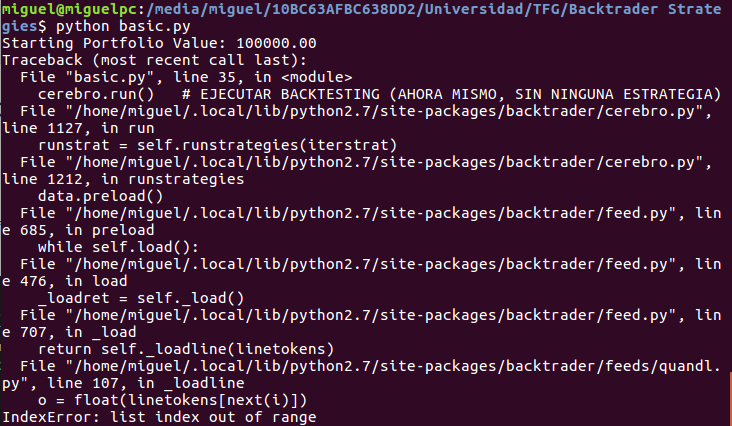
\includegraphics[scale=1.2]{imagenes/quandl_install.png}
				\caption[Ejecuci\'on del script recolectando datos de Quandl]{Ejecuci\'on del script recolectando datos de Quandl. \\Fuente: elaboraci\'on propia.}
				\label{fig:quandl_install}
			\end{figure}
			
			
		\subsubsection{YAHOO! Finance}
				
		Una de las opciones m\'as completas para conseguir los datos es la p\'agina web de \textit{YAHOO! Finance} \footnote{\url{https://finance.yahoo.com}}. Basta con buscar el \'indice o la empresa sobre la que se desean obtener los datos, indicar las fechas y la frecuencia de muestreo y pinchar en el bot\'on de descarga. A continuaci\'on, los datos se descargar\'an en formato CSV con las columnas de fecha, apertura, clausura, m\'aximo, m\'inimo y volumen. Este formato es ampliamente utilizado por la comunidad cient\'ifica para almacenar grandes cantidades de datos.\\
				
		\begin{figure}[H]
			\centering\leftskip=-30px
			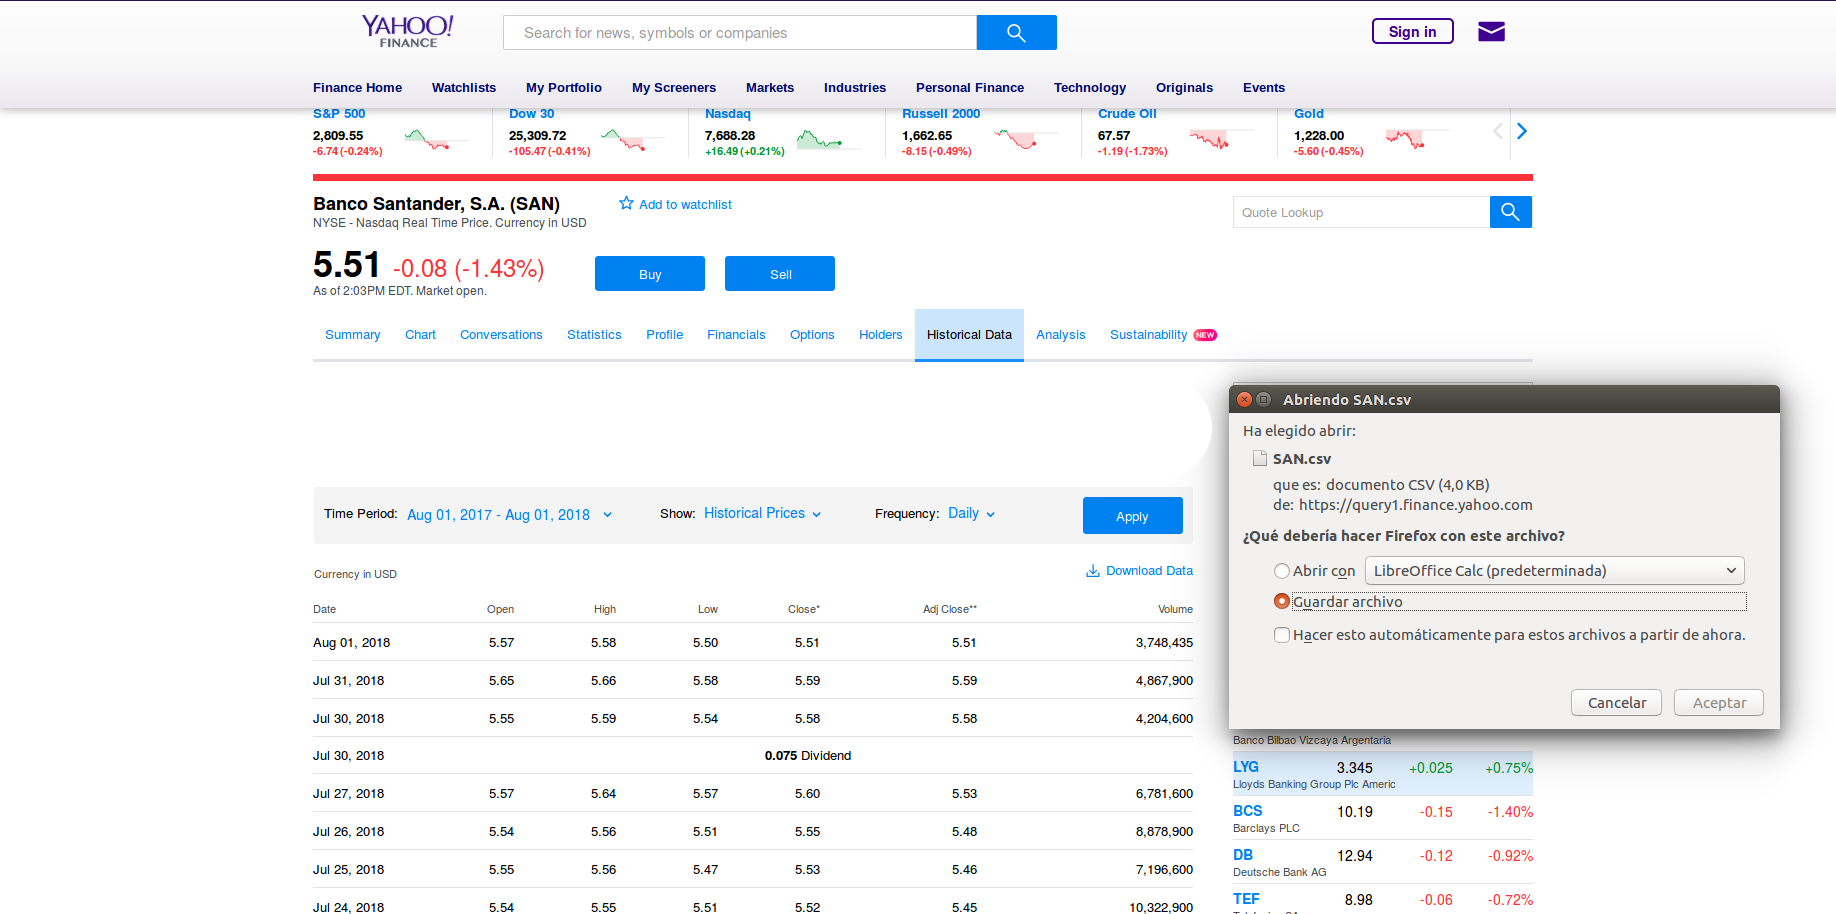
\includegraphics[scale=1]{imagenes/yahoo_finance.png}
			\caption[Descarga de los datos hist\'oricos con \textit{Yahoo! Finance}]{Descarga de los datos hist\'oricos de \textit{Banco Santander}. \\ Fuente: elaboraci\'on propia.}
			\label{fig:yahoo_finance}
		\end{figure}
				
		Por ejemplo, imaginemos que buscamos los valores hist\'oricos de \textit{Banco Santander} desde el 1 de agosto de 2017 hasta la misma fecha del a\~{n}o siguiente. Para ello indicamos la empresa, buscamos el apartado de \textit{Historical Data} e indicamos las fechas. El resultado se muestra en la figura \ref{fig:yahoo_finance}.\\
		
		Finalmente, para cargar estos datos en \textit{backtrader} basta con indicar la ruta donde se encuentra el archivo en el ordenador y el rango de fechas que se quiere ejecutar con el siguiente c\'odigo:\\
		

		\begin{lstlisting}[basicstyle=\tiny]
   # Crear un paquete de datos con YAHOO FINANCE
   data = bt.feeds.YahooFinanceCSVData(
	   dataname='Data/SAN.csv',
	   fromdate=datetime.datetime(2017, 8, 1),
	   todate=datetime.datetime(2018, 8, 1),
	   reverse=False)
   
   # Activar los datos en el cerebro
   cerebro.adddata(data)
		\end{lstlisting}

		Aunque en principio carece de inter\'es, el rango de fechas que se indique debe estar contenido en el archivo, pero no tiene por qu\'e ser el mismo. Este hecho permite descargar y almacenar grandes cantidades de datos, previo a su uso, y almacenarlas para un futuro.\\
		
		Esta opci\'on para adquirir datos es sencilla al tener interfaz gr\'afica, pero no se recomienda si se requiere ejecutar muchas veces con distintas empresas. Por tanto, queda descartado su uso por el momento.


    \subsubsection{Pandas Datareader}
    De forma alternativa a la descarga de CSV anterior, podemos utilizar el paquete \textit{Pandas-datareader}, que proporciona una funci\'on que automatiza la descarga de datos de \textit{YAHOO! Finance}.\\ 
    
    Aunque estuvo un tiempo en desuso y en su documentaci\'on est\'a marcado as\'i\footnote{\url{https://pandas-datareader.readthedocs.io/en/stable/whatsnew.html\#v0-6-0-january-24-2018} [\'Ultima consulta 20 de Julio de 2019]}, ahora vuelve a estar operativo. La \textit{API} de \textit{YAHOO! Finance} cambi\'o y, durante un tiempo, \textit{Pandas-datareader} no la actualiz\'o. No obstante, el tratamiento de los datos por parte de \textit{Pandas-datareader} ya se ha adaptado, aunque no se vea reflejado a\'un en su documentaci\'on.\\
    
    Por nuestra parte, porcomodidad, usaremos a partir de ahora la siguiente f\'ormula para cargar los datos en \textit{Backtrader}:\\
    
    \begin{lstlisting}[basicstyle=\tiny]
    start_date = "2013-08-01"
    end_date   = "2014-02-26"
    simudatos = pdr.get_data_yahoo("SAN", start=start_date, end=end_date)
    df_cerebro = bt.feeds.PandasData(dataname = simudatos)
    \end{lstlisting}
    
    Como puede observarse en el c\'odigo, basta llamar a la funci\'on con el s\'imbolo de la empresa y las fechas de inicio y fin para descargar los datos diarios. N\'otese que la descarga se realiza desde el propio script y es necesaria realizarla en cada ejecuci\'on, pero se hace de forma autom\'atica. Aunque suponga una peque\~na carga para el tiempo, lo usaremos por la  facilidad de cambiar de fechas y empresa.\\
    